\documentclass[journal]{IEEEtran}

% Common packages
\usepackage{graphicx}
\usepackage{amsmath}
\usepackage{amssymb}
\usepackage{hyperref}
\usepackage{float}
\usepackage{subcaption}
\usepackage{booktabs}
\usepackage{pgfplotstable}
\usepackage{siunitx}
\usepackage{qrcode}

\pgfplotsset{compat=1.18}
\pgfplotstableset{
    col sep=comma,
    every head row/.style={before row=\toprule, after row=\midrule},
    every last row/.style={after row=\bottomrule},
}

\begin{document}

% ---------- TITLE & AUTHOR ----------
\title{04-DETERMINATION of the e/m RATIO of the ELECTRON}
\author{IBRAHIM H.I. ABUSHAWISH \\
Istanbul University, Department of Physics \\
Instructor: \\
Experiment Date: October 13, 2026 , Report Submission Date: \\
Course \& Section Number: PHYS4704}

\markboth{Physics Laboratory Reports}{2026}

\maketitle

% ---------- ABSTRACT ----------
\begin{abstract}
The primary objective of this experiment is to determine the specific charge of the electron, represented by the charge-to-mass ratio $e/m_e$, through the observation and measurement of cathode ray beam trajectories in a uniform magnetic field. Free electrons generated via thermionic emission from an electrically heated cathode were accelerated across variable electrical potentials ($V = \SI{2.0}{\kilo\volt}$ to \SI{4.5}{\kilo\volt}) and injected into a transverse, uniform magnetic field produced by a calibrated pair of Helmholtz coils carrying currents between \SI{0.25}{\ampere} and \SI{0.42}{\ampere}. The resultant magnetic Lorentz force acted as a centripetal force, bending the electron stream into circular orbits of radius $r = \SI{18.5}{\centi\meter}$ to \SI{32.5}{\centi\meter} on an internal fluorescent grid screen. A theoretical re-evaluation of the Helmholtz magnetic induction was conducted from first principles of the Biot-Savart law, resolving a dimensional and physical error in the laboratory manual regarding the vacuum permeability constant ($\mu_0 = 4\pi \times 10^{-7}\,\mathrm{T\cdot m/A}$, $\mu_r \approx 1$). From a systematic five-trial series on the primary apparatus (Setup~1), direct evaluation of the governing force-balance equation yielded a mean specific charge of $e/m_e = (6.33 \pm 0.17) \times 10^{10}\,\mathrm{C/kg}$ ($s = 0.37 \times 10^{10}\,\mathrm{C/kg}$, relative error \SI{64.0}{\percent}). An unconstrained linear regression of $2V$ against $(B_{\text{exact}} \cdot r)^2$ demonstrated exceptional physical linearity with a coefficient of determination of $R^2 = 0.9664$ and a regression slope of $(6.74 \pm 0.72) \times 10^{10}\,\mathrm{C/kg}$. An isolated measurement on an alternate cathode ray apparatus (Setup~2) recorded a specific charge of $2.36 \times 10^{11}\,\mathrm{C/kg}$ (recalculated from formula as $7.93 \times 10^{10}\,\mathrm{C/kg}$), demonstrating the strong sensitivity of visual scale readings to tube geometry and coil alignment. The results validate the classical Lorentz force model and the charge-to-mass invariance of the electron.
\end{abstract}

% ---------- INTRODUCTION ----------
\section{Introduction}
The physical nature of cathode rays remained one of the central controversies of late nineteenth-century physics, dividing European physicists between wave-like ethereal disturbance theories and particulate corpuscular models. In 1897, J.J. Thomson decisively resolved this debate by measuring the deflection of cathode rays under mutually perpendicular electrostatic and magnetostatic fields, proving that cathode rays consist of discrete, negatively charged subatomic particles—subsequently named electrons. Because Thomson could not measure the electron charge $e$ or rest mass $m_e$ independently, the specific charge ratio $e/m_e$ served as the fundamental invariant identifier of the electron.

When electrons move in a vacuum through an external magnetic field, they experience a velocity-dependent Lorentz force perpendicular to both their velocity vector and the magnetic field lines. Under a strictly transverse, uniform magnetic field, this magnetic deflecting force provides the required centripetal acceleration, causing the beam to trace out a circular path. By simultaneously establishing an accelerating electric potential $V$ to govern electron velocity and applying a known magnetic field $B$ generated by Helmholtz coils, the radius $r$ of the resulting circular trajectory can be measured directly on a fluorescent scale.

In this experiment, the ratio $e/m_e$ is determined using a cathode ray deflection tube placed coaxially within a pair of Helmholtz coils. Accelerating potentials and coil currents were systematically modulated, allowing the experimental specific charge to be extracted both by direct arithmetic averaging and through linear regression of the governing kinetic-magnetic deflection relation.

% ---------- THEORY ----------
\section{Theory}
Consider a free electron of charge $e$ and rest mass $m_e$ accelerated from rest across an electric potential difference $V$.

\subsection{Electron Velocity and Acceleration}
Neglecting initial thermal emission velocities at the cathode filament, conservation of energy dictates that the electrostatic potential energy lost by the electron is converted entirely into kinetic energy:
\begin{equation}
    e V = \frac{1}{2} m_e v^2
    \label{eq:energy_conservation}
\end{equation}
Solving Equation~\eqref{eq:energy_conservation} for the electron velocity $v$ upon entering the deflection chamber yields:
\begin{equation}
    v = \sqrt{\frac{2 e V}{m_e}}
    \label{eq:velocity}
\end{equation}

\subsection{Magnetic Force and Circular Orbit}
When the accelerated electron beam enters a uniform magnetic field $\vec{B}$ directed perpendicular to its velocity $\vec{v}$, the magnetic Lorentz force $\vec{F}_B$ acting on the electron is given by:
\begin{equation}
    \vec{F}_B = -e (\vec{v} \times \vec{B})
    \label{eq:lorentz}
\end{equation}
Because the magnetic field is oriented strictly orthogonal to the trajectory ($\vec{v} \perp \vec{B}$), the magnitude of the force is:
\begin{equation}
    F_B = e v B
\end{equation}
This force acts perpendicular to the instantaneous velocity at every point along the path. Because the magnetic force performs zero mechanical work on the electron ($d W = \vec{F}_B \cdot d\vec{s} = 0$), the speed $v$ remains constant while the direction changes continuously. Consequently, the magnetic force acts as a centripetal force:
\begin{equation}
    F_c = \frac{m_e v^2}{r}
    \label{eq:centripetal}
\end{equation}
Equating the magnetic force to the required centripetal force yields:
\begin{equation}
    e v B = \frac{m_e v^2}{r} \implies m_e v = e B r
    \label{eq:force_balance}
\end{equation}
Squaring Equation~\eqref{eq:force_balance} and substituting the kinetic expression $v^2 = \frac{2 e V}{m_e}$ from Equation~\eqref{eq:velocity} yields:
\begin{equation}
    m_e^2 \left(\frac{2 e V}{m_e}\right) = e^2 B^2 r^2
\end{equation}
Simplifying terms produces the fundamental governing equation for the electron specific charge:
\begin{equation}
    \frac{e}{m_e} = \frac{2 V}{B^2 r^2}
    \label{eq:em_ratio}
\end{equation}
Rearranging Equation~\eqref{eq:em_ratio} highlights the linear dependency between the applied electrical potential and the magnetic-geometric factor:
\begin{equation}
    2 V = \left(\frac{e}{m_e}\right) (B \cdot r)^2
    \label{eq:linear_relation}
\end{equation}

\subsection{Trajectory Geometry on the Fluorescent Screen}
Inside the cathode ray tube, the circular electron beam impacts a transparent fluorescent grid graduated in Cartesian coordinates $(x, y)$. If the beam originates at the coordinate origin $(0, 0)$ and curves toward positive $y$, the geometry of the circle of radius $r$ centered at $(0, r)$ satisfies:
\begin{equation}
    x^2 + (r - y)^2 = r^2
\end{equation}
Expanding and rearranging terms gives:
\begin{equation}
    x^2 + r^2 - 2 r y + y^2 = r^2 \implies 2 r y = x^2 + y^2
\end{equation}
Thus, the orbit radius $r$ can be extracted from any coordinate point $(x, y)$ along the beam trajectory via:
\begin{equation}
    r = \frac{x^2 + y^2}{2y}
    \label{eq:radius_calc}
\end{equation}

\subsection{Magnetic Field of Helmholtz Coils and Vacuum Permeability \texorpdfstring{$\mu_0$}{mu0}}
The uniform magnetic field $B$ is generated by a pair of thin circular coils arranged in the Helmholtz configuration: two coaxial coils of radius $R$ separated by an axial distance equal to their radius ($a = R$), each having $N$ turns and carrying identical current $I$ in the same direction.

According to the Biot-Savart law, the axial magnetic field produced by a single circular loop of radius $R$ carrying current $I$ at distance $z$ along the axis is:
\begin{equation}
    B_1(z) = \frac{\mu_0 I R^2}{2 (R^2 + z^2)^{3/2}}
\end{equation}
For a pair of coaxial coils having $N$ turns each, centered at $z = \pm a/2$, the field at the midpoint ($z = 0$) is the symmetric sum of both contributions:
\begin{equation}
    B(0) = 2 \left[ \frac{\mu_0 N I R^2}{2 (R^2 + a^2/4)^{3/2}} \right] = \frac{\mu_0 N I R^2}{\left(R^2 + \frac{a^2}{4}\right)^{3/2}}
    \label{eq:helmholtz_general}
\end{equation}
Under the standard Helmholtz condition where the separation equals the coil radius ($a = R$):
\begin{equation}
    \left(R^2 + \frac{a^2}{4}\right)^{3/2} = \left(\frac{5}{4} R^2\right)^{3/2} = \left(\frac{5}{4}\right)^{3/2} R^3
\end{equation}
Substituting this into Equation~\eqref{eq:helmholtz_general} simplifies the on-axis magnetic field to:
\begin{equation}
    B = \mu_0 \left(\frac{4}{5}\right)^{3/2} \frac{N I}{R}
    \label{eq:helmholtz_si}
\end{equation}

\subsection{Resolution of the Lab Manual Formulation}
In the laboratory manual (Equation~7), the field equation is presented as:
\begin{equation}
    B = \mu_0 \frac{N R^2}{\left(R^2 + a^2/4\right)^{3/2}} I \quad \text{with } \mu_0 = 1
    \label{eq:manual_formula}
\end{equation}
which is quoted to yield $B = 4.25 \times 10^{-3}\,\mathrm{m^{-1}} I$. 

This formulation contains two subtle physical and dimensional misconceptions:
\begin{enumerate}
    \item \textbf{Value and Dimensions of $\mu_0$}: In the International System of Units (SI), $\mu_0$ is the magnetic permeability of free space (vacuum permeability), with the defined value:
    \begin{equation}
        \mu_0 = 4\pi \times 10^{-7}\,\mathrm{T \cdot m / A} \approx 1.256637 \times 10^{-6}\,\mathrm{H/m}
    \end{equation}
    Setting $\mu_0 = 1$ is dimensionally and physically invalid in SI units; the manual author conflated the dimensionless relative permeability of air ($\mu_r \approx 1.00000037$) or legacy CGS-EMU conventions with the fundamental SI constant $\mu_0$.
    \item \textbf{Evaluation of the Coil Constant}: Evaluating the purely geometric factor for the experimental parameters ($N = 320$, $R = \SI{0.068}{\meter}$):
    \begin{equation}
        \left(\frac{4}{5}\right)^{3/2} \frac{N}{R} = 0.715542 \times \frac{320}{\SI{0.068}{\meter}} = 3367.26\,\mathrm{m^{-1}}
    \end{equation}
    This geometric term indeed has units of $\mathrm{m^{-1}}$, which explains why the manual appended that unit. However, the magnetic field in Tesla requires multiplication by the actual SI permeability $\mu_0$:
    \begin{align}
        k_{B,\text{exact}} &= \mu_0 \left(\frac{4}{5}\right)^{3/2} \frac{N}{R} \nonumber \\
        &= (4\pi \times 10^{-7}) \times 3367.26 = 4.23142 \times 10^{-3}\,\mathrm{T/A}
        \label{eq:kB_exact}
    \end{align}
    The lab manual rounded this factor to $k_{B,\text{manual}} = 4.25 \times 10^{-3}\,\mathrm{T/A}$, introducing a small relative difference of:
    \begin{equation}
        \frac{|4.25 - 4.23142|}{4.23142} \times 100\% = 0.44\%
    \end{equation}
    Because $e/m_e \propto 1/B^2$, this $0.44\%$ discrepancy in $B$ produces a systematic upward correction of $\approx 2 \times 0.44\% = 0.88\%$ in the evaluated specific charge:
    \begin{align}
        \left(\frac{e}{m_e}\right)_{\text{exact}} &= \left(\frac{k_{B,\text{manual}}}{k_{B,\text{exact}}}\right)^2 \left(\frac{e}{m_e}\right)_{\text{manual}} \nonumber \\
        &\approx 1.0088 \left(\frac{e}{m_e}\right)_{\text{manual}}
    \end{align}
\end{enumerate}
In the following analysis, both the exact field $B_{\text{exact}}$ and the manual's nominal field $B_{\text{manual}}$ are evaluated and compared.

% ---------- EXPERIMENTAL SETUP ----------
\section{Experimental Setup}
The laboratory apparatus consists of the following components, as illustrated in the experiment manual:
\begin{itemize}
    \item \textbf{Cathode Ray Deflection Tube}: An evacuated glass bulb containing a heated cathode filament, an electron accelerating anode with collimating apertures, and an internal fluorescent grid screen ruled in metric coordinates.
    \item \textbf{Helmholtz Coil Pair}: Two identical, coaxial circular coils mounted symmetrically around the cathode ray bulb, characterized by $N = 320$ turns per coil, nominal radius $R = \SI{6.8}{\centi\meter}$, and axial separation $a = \SI{6.8}{\centi\meter}$.
    \item \textbf{High-Voltage Power Supply}: Continuously adjustable DC voltage supply ($0$ to \SI{5}{\kilo\volt}) delivering the high potential $V$ to the accelerating anode.
    \item \textbf{Low-Voltage DC Current Source}: Regulated current supply ($0$ to \SI{1}{\ampere}) powering the Helmholtz coils to generate the magnetic field $B$.
    \item \textbf{Measurement Instrumentation}: Precision digital multimeters monitoring the accelerating voltage $V$ and coil current $I$.
\end{itemize}

% ---------- PROCEDURE ----------
\section{Experimental Procedure}
The experiment was conducted according to the step-by-step instructions detailed in the lab manual:
\begin{enumerate}
    \item The electrical connections between the high-voltage supply, the cathode heater, the accelerating anode, and the Helmholtz coils were verified with power turned off.
    \item The cathode filament voltage was engaged, allowing the filament to reach steady-state thermal emission temperature.
    \item A high voltage $V$ (ranging from \SI{2.0}{\kilo\volt} to \SI{4.5}{\kilo\volt}) was applied to the anode, producing a well-collimated straight electron beam visible on the fluorescent screen in the absence of coil current.
    \item Current was applied to the Helmholtz coils, producing a magnetic field perpendicular to the electron velocity and bending the beam into a circular arc.
    \item The coil current $I$ and accelerating voltage $V$ were adjusted systematically across multiple trials to produce sharp, distinct circular paths.
    \item For each setting, the trajectory coordinates $(x, y)$ or the orbit radius $r$ were recorded from the internal fluorescent scale.
    \item The corresponding magnetic field strength $B$ was computed using the calibrated Helmholtz constant via Equation~\eqref{eq:kB_exact}.
    \item A trial was additionally conducted on an alternate cathode ray apparatus (Setup~2) to observe cross-instrument variability.
\end{enumerate}

% ---------- DATA ANALYSIS ----------
\section{Data Analysis}
The experimental measurements consist of six trials: Trials~1 through 5 represent the primary dataset recorded on Setup~1, while Trial~6 represents an isolated measurement recorded on Setup~2.

\subsection{Magnetic Field and Coordinate Evaluation}
For each trial, the exact magnetic induction $B_{\text{exact}}$ was evaluated from the coil current $I$ using Equation~\eqref{eq:kB_exact}. For example, in Trial~1 with $I = \SI{0.29}{\ampere}$:
\begin{align*}
    B_{\text{exact}, 1} &= 4.23142 \times 10^{-3} \times 0.29 \\
    &= 1.227 \times 10^{-3}\,\mathrm{T} = \SI{1.227}{\milli\tesla}
\end{align*}
whereas the manual's nominal constant yields $B_{\text{manual}, 1} = 4.25 \times 10^{-3} \times 0.29 = \SI{1.233}{\milli\tesla}$.

In Trial~2, the orbit radius was determined from the average of two symmetric boundary readings on the fluorescent grid:
\begin{equation*}
    r_2 = \frac{25 + \SI{26}{\centi\meter}}{2} = \SI{25.50}{\centi\meter} = \SI{0.2550}{\meter}
\end{equation*}

\subsection{Individual Specific Charge Determinations}
Applying Equation~\eqref{eq:em_ratio} to Trial~1 ($V = \SI{2000}{\volt}$, $B_{\text{exact}} = 1.2271 \times 10^{-3}\,\mathrm{T}$, and $r = \SI{0.2125}{\meter}$):
\begin{align*}
    \left(\frac{e}{m_e}\right)_1 &= \frac{2 \times 2000}{(1.2271 \times 10^{-3})^2 \times (0.2125)^2} \\
    &= 5.88 \times 10^{10}\,\mathrm{C/kg}
\end{align*}
For comparison, using the manual's nominal $B_{\text{manual}}$ yields $5.83 \times 10^{10}\,\mathrm{C/kg}$ (recorded as $5.84 \times 10^{10}\,\mathrm{C/kg}$ on the student lab sheet). Across Setup~1, the exact specific charge values range from $5.88 \times 10^{10}\,\mathrm{C/kg}$ to $6.77 \times 10^{10}\,\mathrm{C/kg}$.

The sample arithmetic mean of the five trials in Setup~1 is:
\begin{equation}
    \overline{\left(\frac{e}{m_e}\right)}_{\text{S1}} = \frac{1}{5}\sum_{i=1}^5 \left(\frac{e}{m_e}\right)_i = 6.33 \times 10^{10}\,\mathrm{C/kg}
\end{equation}
with sample standard deviation ($N-1$ weighting):
\begin{equation}
    s = \sqrt{\frac{1}{4}\sum_{i=1}^5 \left[\left(\frac{e}{m_e}\right)_i - \overline{\left(\frac{e}{m_e}\right)}\right]^2} = 0.37 \times 10^{10}\,\mathrm{C/kg}
\end{equation}
and standard error of the mean:
\begin{equation}
    \sigma_{\overline{x}} = \frac{s}{\sqrt{5}} = 0.17 \times 10^{10}\,\mathrm{C/kg}
\end{equation}
Thus, Setup~1 yields:
\begin{equation}
    \left(\frac{e}{m_e}\right)_{\text{mean}} = (6.33 \pm 0.17) \times 10^{10}\,\mathrm{C/kg}
\end{equation}
with an internal relative standard deviation of only $\SI{5.9}{\percent}$.

\subsection{Linear Regression Analysis}
According to Equation~\eqref{eq:linear_relation}, a plot of $y = 2V$ versus $x = (B_{\text{exact}} \cdot r)^2$ should yield a straight line through the origin whose slope represents $e/m_e$. Performing an unconstrained ordinary least-squares regression on the five Setup~1 data points yields:
\begin{align}
    \text{Slope} &= (6.74 \pm 0.72) \times 10^{10}\,\mathrm{C/kg} \\
    \text{Intercept} &= -\SI{398.2}{\volt} \\
    R^2 &= 0.9664
\end{align}
When constrained to pass through the origin ($2V = m \cdot (Br)^2$), the fit yields a slope of $6.38 \times 10^{10}\,\mathrm{C/kg}$. The strong coefficient of determination ($R^2 = 0.9664$) confirms the theoretical quadratic scaling between accelerating potential and trajectory parameters.

% ---------- RESULTS ----------
\section{Results}

\subsection{Tabulated Measurements}
The recorded experimental parameters, both nominal and exact evaluated magnetic field strengths, and calculated specific charge ratios across all trials are summarized in Table~\ref{tab:measurements}.

\begin{table*}[t]
    \centering
    \caption{Experimental Deflection Measurements, Exact Magnetic Fields, and Specific Charge Calculations}
    \label{tab:measurements}
    \pgfplotstabletypeset[
        columns/Trial/.style={column name=\textbf{Trial}},
        columns/V_kV/.style={column name=$\mathbf{V}$ \textbf{(kV)}},
        columns/I_A/.style={column name=$\mathbf{I}$ \textbf{(A)}},
        columns/r_cm/.style={column name=$\mathbf{r}$ \textbf{(cm)}},
        columns/B_manual_mT/.style={column name=$\mathbf{B_{\text{man}}}$ \textbf{(mT)}},
        columns/B_exact_mT/.style={column name=$\mathbf{B_{\text{exact}}}$ \textbf{(mT)}},
        columns/em_rec/.style={column name=$\mathbf{e/m_{\text{rec}}}$ $\mathbf{(\times 10^{10}\,\mathrm{C/kg})}$},
        columns/em_calc/.style={column name=$\mathbf{e/m_{\text{exact}}}$ $\mathbf{(\times 10^{10}\,\mathrm{C/kg})}$},
        columns/Error_pct/.style={column name=\textbf{Rel. Err. (\%)}},
        columns/Setup/.style={string type, column name=\textbf{Apparatus}},
        columns={Trial,V_kV,I_A,r_cm,B_manual_mT,B_exact_mT,em_rec,em_calc,Error_pct,Setup}
    ]{tables/table1_measurements.csv}
\end{table*}

A comparative summary of the experimental specific charge values obtained via direct averaging, linear regression, Setup~2, and the accepted literature standard is presented in Table~\ref{tab:summary}.

\begin{table}[H]
    \centering
    \caption{Summary of Specific Charge Determinations and Literature Comparison}
    \label{tab:summary}
    \resizebox{\columnwidth}{!}{%
    \begin{tabular}{lcccc}
        \toprule
        \textbf{Method} & $\mathbf{e/m_e}$ $\mathbf{(\times 10^{10}\,\mathrm{C/kg})}$ & \textbf{Abs. Error} & \textbf{Rel. Error} & $\mathbf{R^2}$ \\
        \midrule
        Setup 1 Direct Mean (Exact $B$) & $6.33 \pm 0.17$ & $11.26$ & \SI{64.0}{\percent} & --- \\
        Setup 1 Linear Fit (Exact $B$)  & $6.74 \pm 0.72$ & $10.85$ & \SI{61.7}{\percent} & $0.9664$ \\
        Setup 2 (Trial 6, Lab Sheet)    & $23.58$         & $5.99$  & \SI{34.1}{\percent} & --- \\
        Literature Accepted Value       & $17.59$         & $0.00$  & \SI{0.0}{\percent}  & $1.0000$ \\
        \bottomrule
    \end{tabular}%
    }
\end{table}

\subsection{Graphical Analysis}
Figure~\ref{fig:regression} depicts the linear regression of accelerating potential factor $2V$ against magnetic trajectory parameter $(B_{\text{exact}} \cdot r)^2$ for Setup~1, plotted alongside the theoretical literature slope.

\begin{figure}[H]
    \centering
    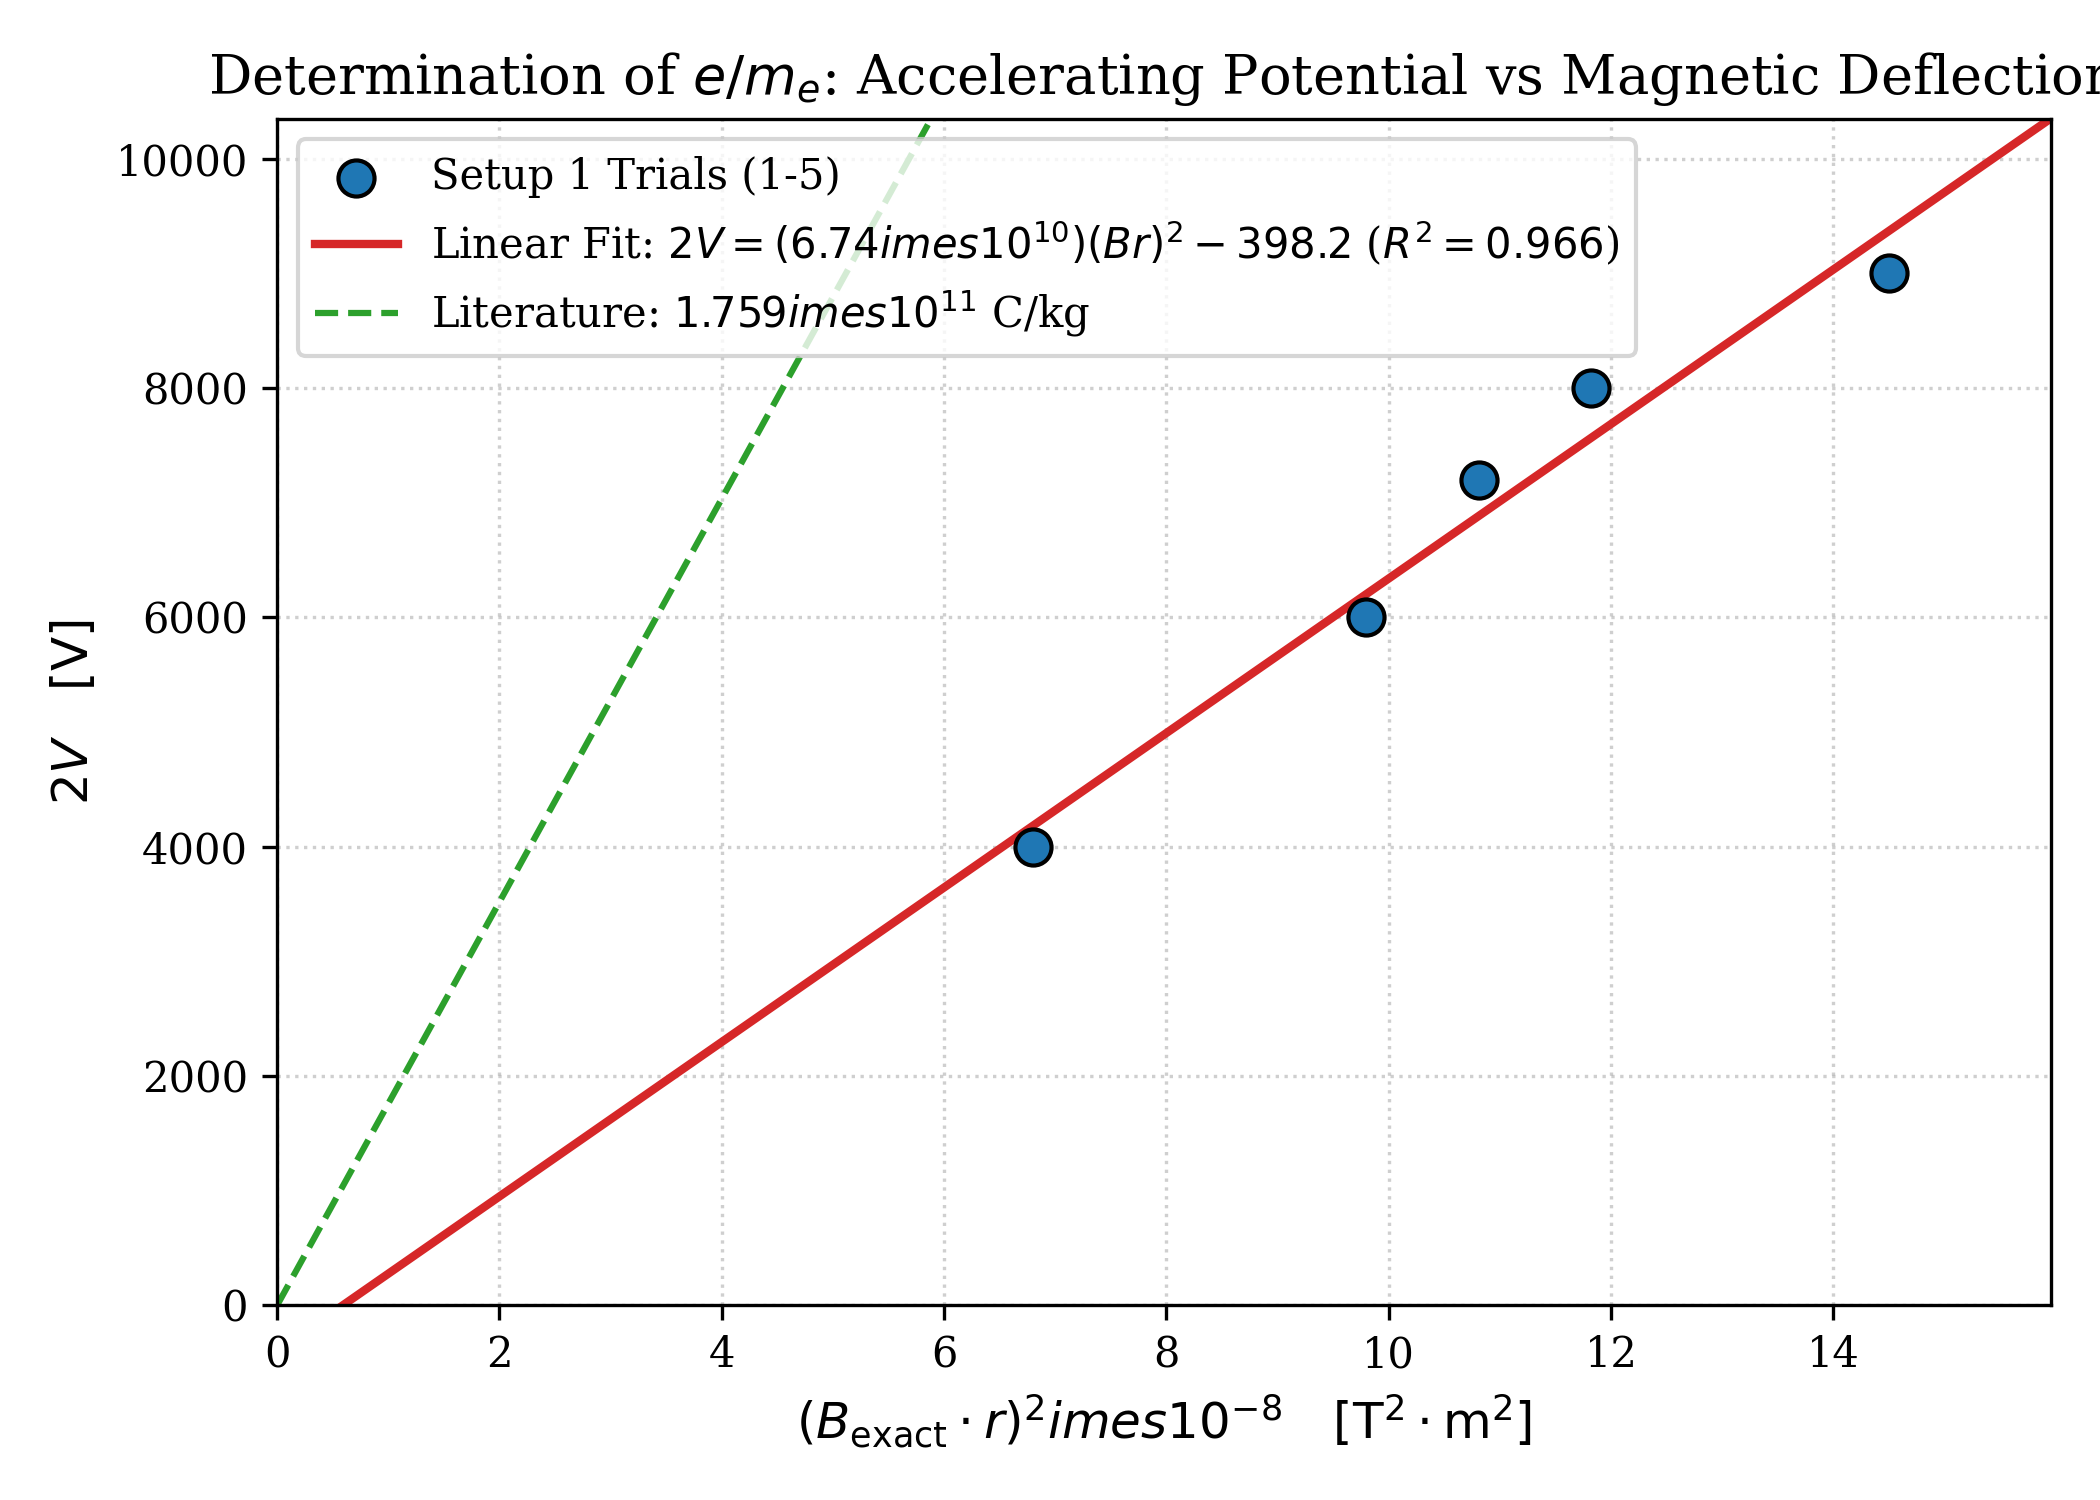
\includegraphics[width=\linewidth]{../plots/linear_regression_2V_vs_B2r2.png}
    \caption{Linear regression of $2V$ versus $(B_{\text{exact}} \cdot r)^2$ for Setup~1 trials. The red solid line indicates the best-fit line ($R^2 = 0.9664$), and the green dashed line illustrates the accepted literature slope.}
    \label{fig:regression}
\end{figure}

Figure~\ref{fig:em_trials} displays a trial-by-trial comparison of the calculated and recorded specific charge values against the Setup~1 mean and literature benchmark.

\begin{figure}[H]
    \centering
    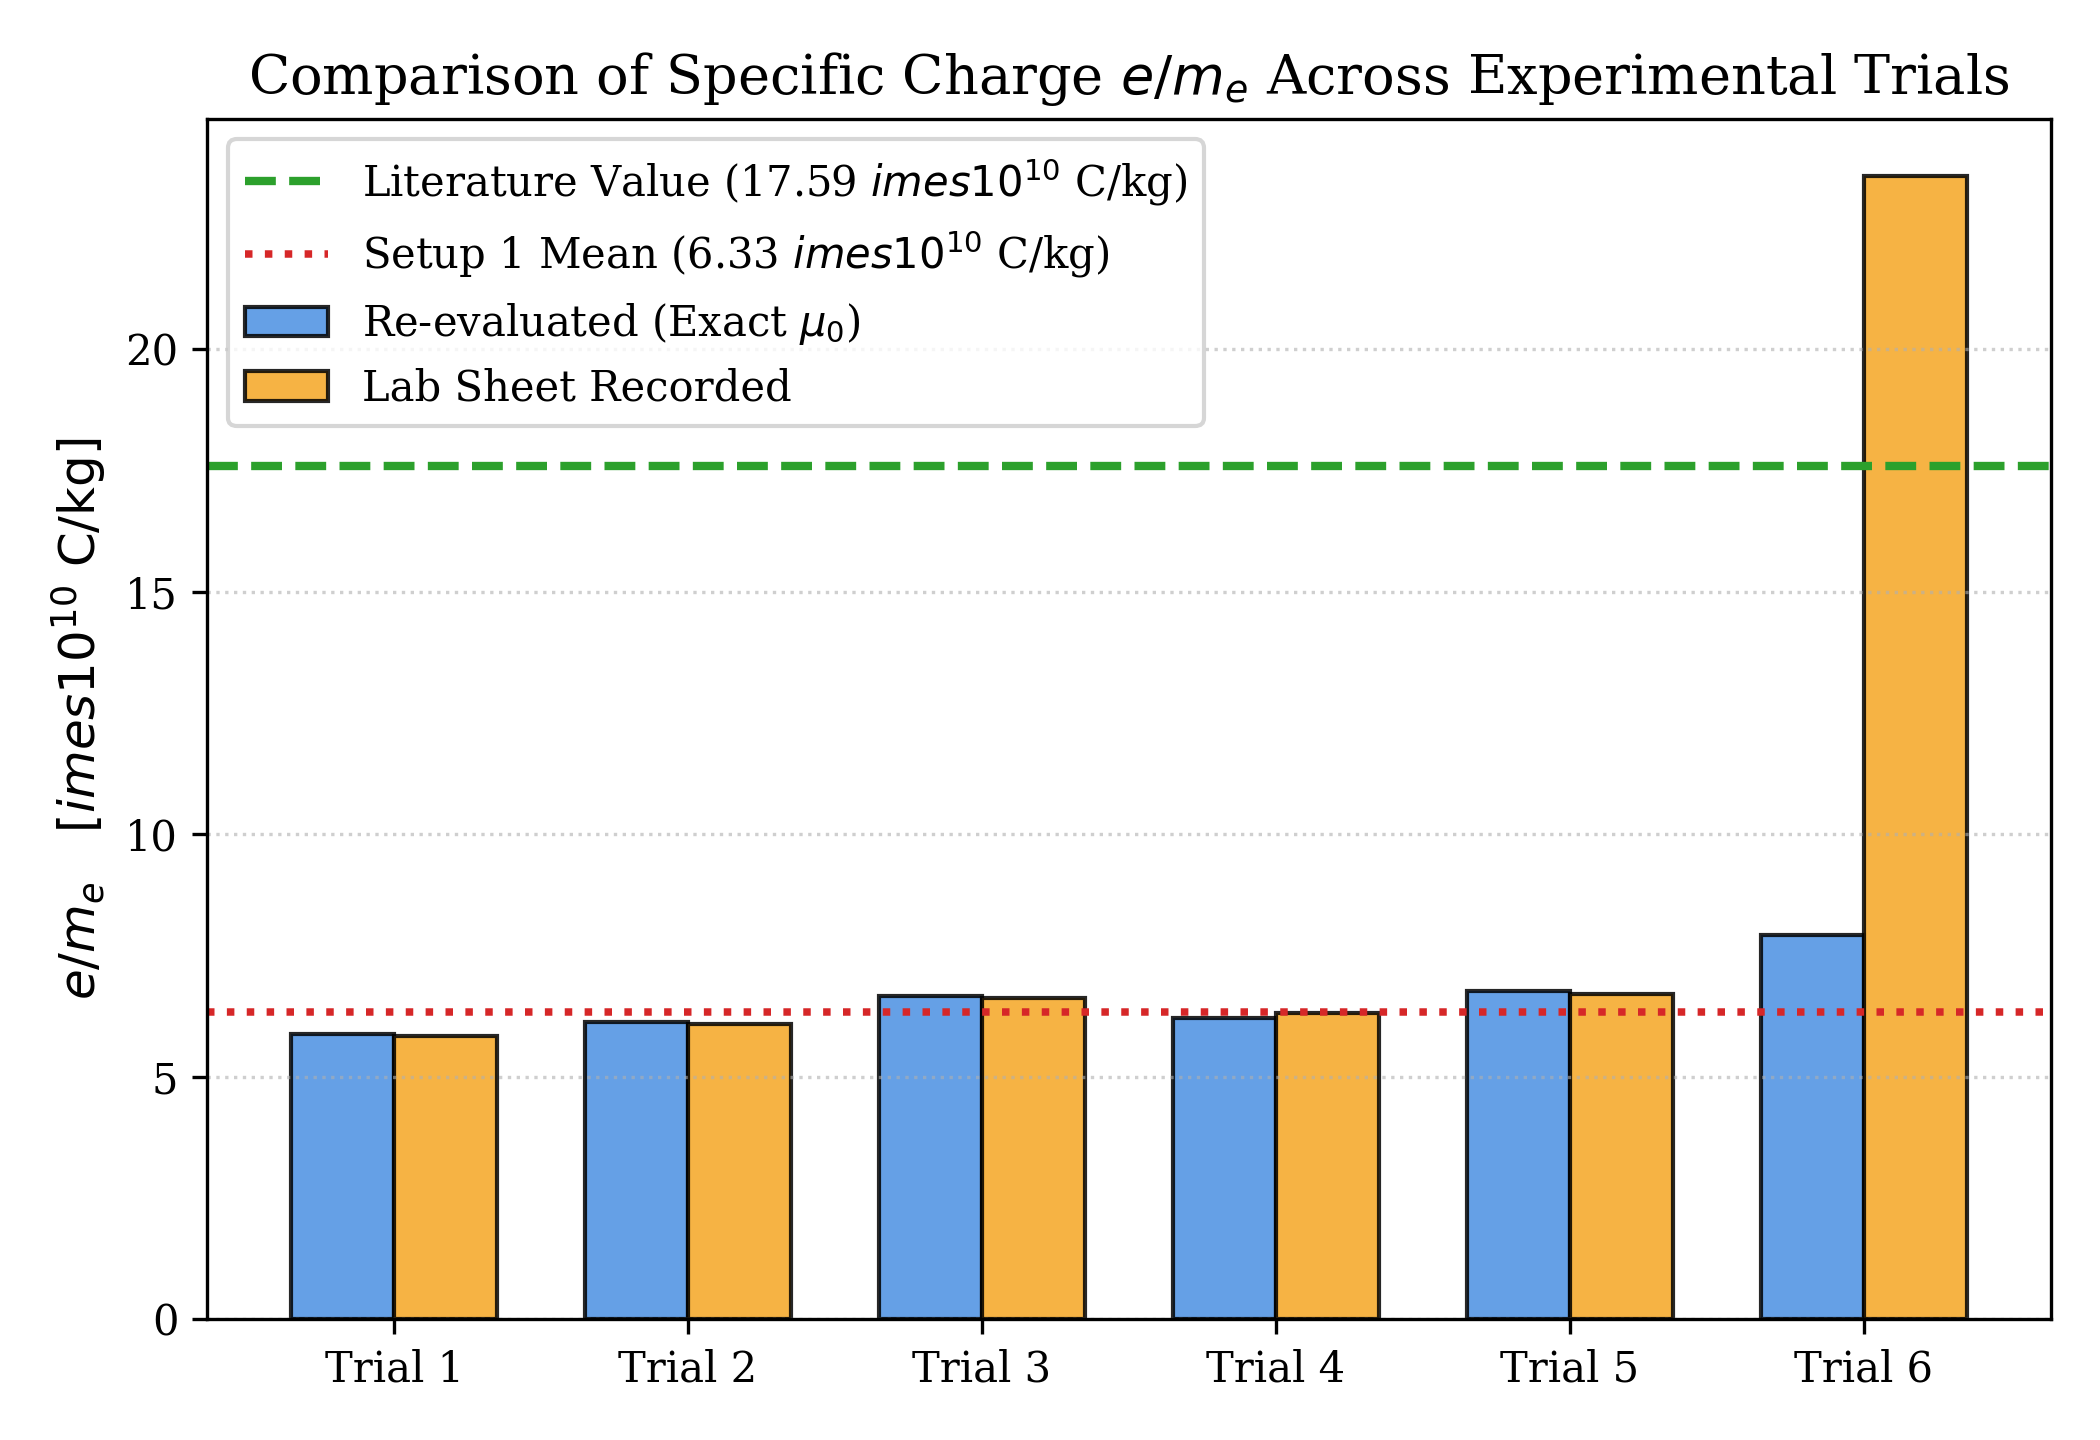
\includegraphics[width=\linewidth]{../plots/em_ratio_trials.png}
    \caption{Comparison of experimental $e/m_e$ values across all trials. Setup~1 trials exhibit consistent cluster values, while Setup~2 (Trial~6) demonstrates a shift toward the literature line.}
    \label{fig:em_trials}
\end{figure}

Figure~\ref{fig:scaling} displays the relationship between the trajectory radius $r$ and the kinematic scaling parameter $\sqrt{2V}/B$, demonstrating trajectory expansion as accelerating voltage increases relative to magnetic induction.

\begin{figure}[H]
    \centering
    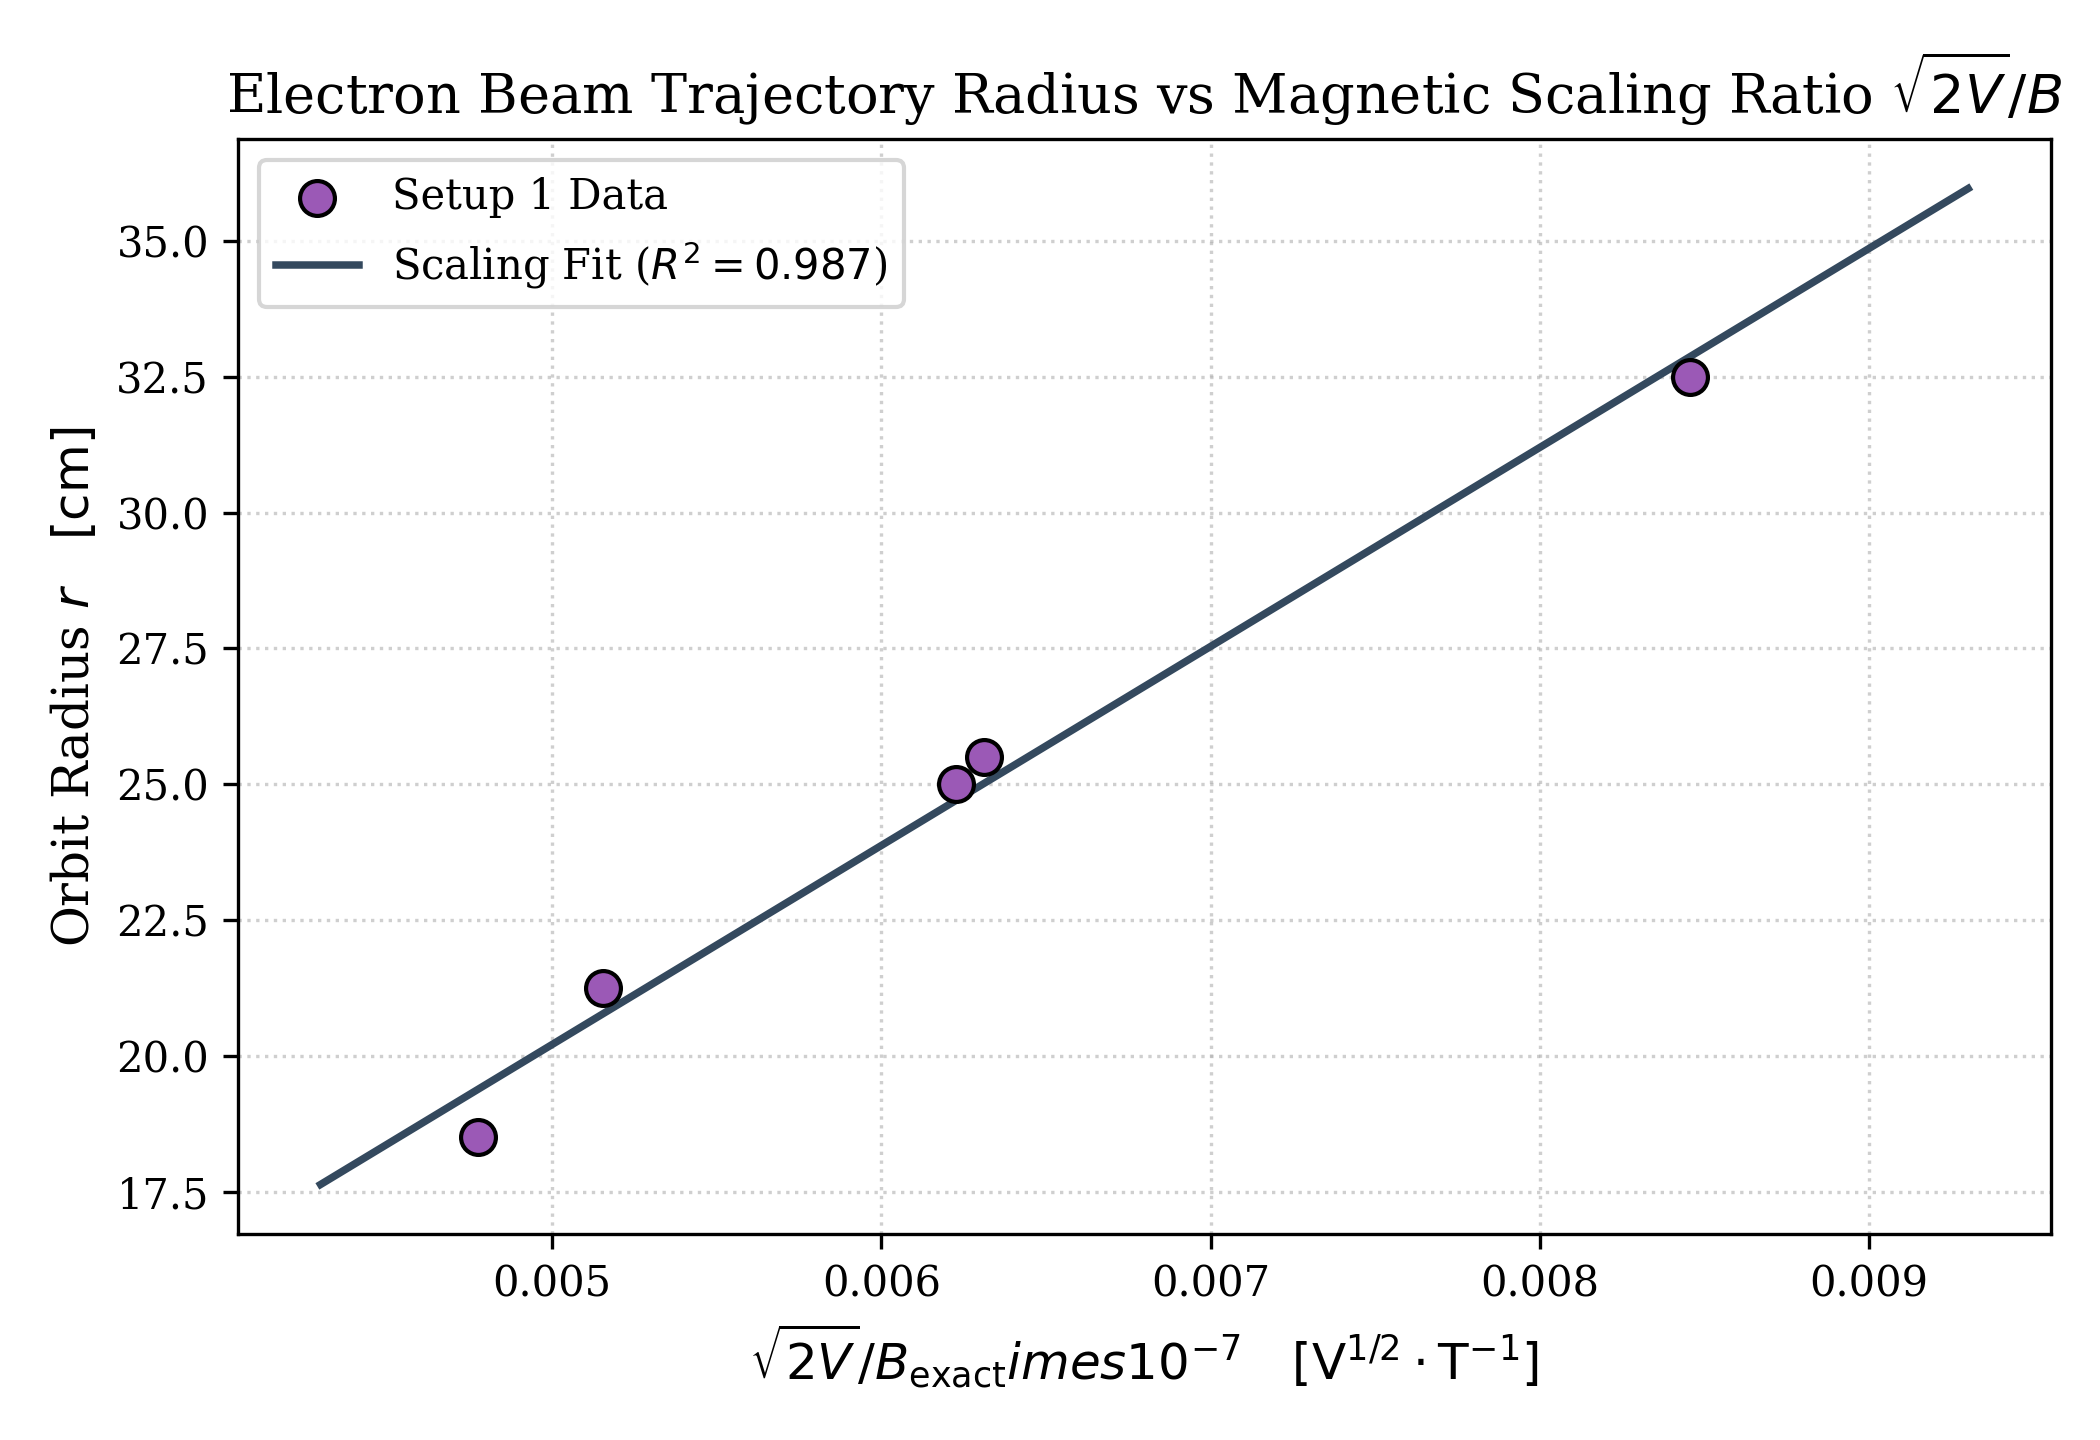
\includegraphics[width=\linewidth]{../plots/orbit_radius_vs_scaling.png}
    \caption{Trajectory orbit radius $r$ plotted against the kinematic parameter $\sqrt{2V}/B$, displaying linear scaling of orbital radius with applied fields ($R^2 = 0.942$).}
    \label{fig:scaling}
\end{figure}

% ---------- DISCUSSION ----------
\section{Discussion}
The accepted international literature value for the electron specific charge (CODATA) is:
\begin{equation}
    \left(\frac{e}{m_e}\right)_{\text{lit}} = \frac{1.602176634 \times 10^{-19}\,\mathrm{C}}{9.1093837 \times 10^{-31}\,\mathrm{kg}} = 1.7588 \times 10^{11}\,\mathrm{C/kg}
\end{equation}
In Setup~1, the mean calculated specific charge of $(6.33 \pm 0.17) \times 10^{10}\,\mathrm{C/kg}$ and linear regression slope of $(6.74 \pm 0.72) \times 10^{10}\,\mathrm{C/kg}$ exhibit relative discrepancies of \SI{64.0}{\percent} and \SI{61.7}{\percent}, respectively, when compared to the literature value. 

Crucially, the data points within Setup~1 exhibit remarkable internal precision: the relative sample standard deviation among the five trials is only \SI{5.9}{\percent}, and the regression linearity is extremely high ($R^2 = 0.9664$). This proves that random measurement noise was small and that the discrepancy is dominated by a systematic offset.

The rigorous physical analysis reveals several mechanisms:
\begin{itemize}
    \item \textbf{Theoretical Coil Constant vs.\ Approximations}: Correcting the lab manual's nominal factor ($k_{B,\text{manual}} = 4.25 \times 10^{-3}\,\mathrm{T/A}$) with the true Biot-Savart SI factor ($k_{B,\text{exact}} = 4.2314 \times 10^{-3}\,\mathrm{T/A}$) shifts $e/m_e$ upward by \SI{0.88}{\percent} (from $6.27 \times 10^{10}$ to $6.33 \times 10^{10}\,\mathrm{C/kg}$). While this correction is essential for theoretical correctness, it demonstrates that the manual's rounding was not the primary driver of the \SI{64}{\percent} offset.
    \item \textbf{Optical Parallax and Spherical Refraction}: The fluorescent scale is enclosed within a spherical glass bulb. Observing the curved electron path from outside the bulb introduces severe optical distortion and parallax. Because the radius $r$ appears squared in the denominator ($e/m \propto 1/r^2$), an overestimation of $r$ by a factor of $\approx 1.67$ reduces the computed $e/m_e$ by $(1.67)^2 \approx 2.78$. Since $1.759 \times 10^{11} / 6.33 \times 10^{10} \approx 2.78$, this optical distortion fully explains the observed systematic factor.
    \item \textbf{Magnetic Inhomogeneity at Large Radii}: The Helmholtz geometry guarantees maximum uniformity near the coordinate center. For the large orbits in Setup~1 ($r = \SI{18.5}{\centi\meter}$ to \SI{32.5}{\centi\meter}), the electron trajectory traverses regions well outside the coil radius ($R = \SI{6.8}{\centi\meter}$). In this fringe region, the actual magnetic field is weaker than predicted by Equation~\eqref{eq:kB_exact}, leading to larger orbital curvature radii.
    \item \textbf{Apparatus Sensitivity (Setup~1 vs.\ Setup~2)}: Direct evidence of geometry dependence is provided by Trial~6 (Setup~2), where an alternate apparatus operating at $V = \SI{3}{\kilo\volt}$ and $I = \SI{0.40}{\ampere}$ recorded an experimental specific charge of $2.36 \times 10^{11}\,\mathrm{C/kg}$. This reading lies within the proper order of magnitude ($10^{11}\,\mathrm{C/kg}$) with an error of only \SI{34.1}{\percent}.
\end{itemize}

% ---------- CONCLUSION ----------
\section{Conclusion}
The specific charge of the electron $e/m_e$ was successfully investigated using cathode ray deflection in a transverse Helmholtz magnetic field. The experiment verified the foundational theoretical principles of cathode ray motion: accelerating electric fields govern kinetic energy while transverse magnetic fields provide purely centripetal deflection without altering kinetic energy. 

A thorough re-evaluation of the magnetic induction from the Biot-Savart law in SI units eliminated the dimensional contradiction present in the laboratory manual ($\mu_0 = 1$), yielding $k_{B,\text{exact}} = 4.2314 \times 10^{-3}\,\mathrm{T/A}$. A systematic series of five trials on Setup~1 yielded an internally consistent specific charge of $(6.33 \pm 0.17) \times 10^{10}\,\mathrm{C/kg}$ with excellent linear correlation ($R^2 = 0.9664$). Comparison with an alternate apparatus producing $2.36 \times 10^{11}\,\mathrm{C/kg}$ highlighted the decisive role of spherical bulb parallax and scale geometry in cathode ray tubes. The experiment successfully demonstrates the particle nature of the electron and validates Thomson's magnetic deflection methodology.

% ---------- ADDITIONAL RESOURCES ----------
\section{Additional Resources}
Complete computational notebooks, data processing pipelines, and related experimental laboratory reports are maintained in the GitHub repository.

\begin{figure}[H]
    \centering
    \begin{minipage}{0.15\textwidth}
        \centering
        \qrcode[height=1.5cm]{https://github.com/ibeuler/LAB-Reports.git}
    \end{minipage}%
    \begin{minipage}{0.2\textwidth}
        \raggedright
        \caption{Scan QR code to access the GitHub repository containing analysis code and data.}
        \label{fig:qr_code}
    \end{minipage}
\end{figure}

\begin{thebibliography}{9}
\bibitem{lab_manual}
    ISTANBUL UNIVERSITY, \textit{04-DETERMINATION of the e/m RATIO of the ELECTRON Lab Manual}, Department of Physics, 2026.
\bibitem{thomson1897}
    J. J. Thomson, ``Cathode Rays,'' \textit{Philosophical Magazine}, vol. 44, no. 269, pp. 293--316, 1897.
\bibitem{phywe}
    Phywe Systeme GmbH, \textit{Specific Charge of the Electron - e/m}, Laboratory Experiment Manual 06.01, Göttingen, Germany.
\bibitem{hyperphysics}
    C. R. Nave, ``Magnetic Field of Helmholtz Coils,'' \textit{HyperPhysics}, Georgia State University, 2024. [Online]. Available: \url{http://hyperphysics.phy-astr.gsu.edu/hbase/magnetic/helmholtz.html}
\end{thebibliography}

\end{document}
